% !TeX root = ../main.tex
\chapter{基于SVM的股票价格预测模型实验}

\section{实验环境}

\subsection{硬件环境}

内存:16.00 GB

CPU:Intel(R) Core(TM) i7-1065G7 CPU @ 1.30GHZ 1.50GHz。

\subsection{软件环境}
本文使用的软件环境如下表:
\begin{table}[ht]
    \centering
    \caption{软件(包)版本}
    \begin{tabular}{lc}
        \hline
        {名称} & {版本号}\\
        \hline
        {Linux (WSL)} & {4.19.104-microsoft-standard}\\
        {Python} & {3.7.7}\\
        {Numpy} & {1.81.1}\\
        {Pandas} & {1.0.3}\\
        {Scikit-learn} & {0.22.1}\\
        {Hyperopt} & {0.2.3}
    \end{tabular}
\end{table}

\section{实验流程}

实验过程中,所有涉及随机过程的随机数生成器的种子均为$42$。

\subsubsection{数据预处理}

在数据输入模型之前,还需要进行数据预处理。
首先我们利用train\underline{~~}test\underline{~~}split函数来随机地将数据分割成4个部分,
X\underline{~~}train代表的是训练样本的输入向量的数据,即选择的相关指标,包括Open\underline{~~}up,Close\underline{~~}up等等;
y\underline{~~}train代表的是训练样本的输出向量的数据,即未来$T$个交易日的平均最低价T\underline{~~}mean;
X\underline{~~}test代表的是测试样本的输入向量的数据;
y\underline{~~}test代表的是测试样本的输出向量的数据;
然后,经过多次测试,使用$Z\text{-}score$方法来对数据进行标准化,
这里使用的是StandardScaler类来对X\underline{~~}train和X\underline{~~}test进行标准化,
需要注意的是StandardScaler类不能对所有样本进行适配,因为测试样本不应该包含任何关于训练数据的先验信息。

\subsubsection{超参数寻优}

基于前人的经验和多次实验的检验,本文最终选择了RBF核函数,能够取得更平滑的估计,其中$\gamma$的值决定了模型的收敛速度,
$\gamma$越小,收敛越快。但是小的$\gamma$值带来的问题是,所有的预测结果都将接近于平均值,$MSE$虽然不大但是预测结果没有任何参考意义。
所以找到一组好的参数能够使模型的预测效果更好。

此处我们利用KFold函数来将训练数据随机地分成5份来进行交叉验证,将输出的平均均方误差来作为超参数寻优最小化的目标,
再利用Hyperopt包定义超参数搜寻空间$(C,\gamma)\in[1, 1000]\times[0.00001, 0.1]$,
并利用Hyperopt提供的TPE算法来进行超参数寻优,其中迭代次数设定为$200$次。

\section{实验结果与分析}

按照上述过程,对$T=2\sim15$和日线\underline{~~}1、日线\underline{~~}2、周线\underline{~~}1、周线\underline{~~}2共56种情况进行实验,得到结果如下:

\subsection{日线第1种情况}

表(4.3)中给出了日线\underline{~~}1的实验结果,可以看到相差无几的数据集输入模型后所产生的超参数黑盒函数也是不尽相同的,
$MSE$是衡量模型预测效果的重要指标,由$MSE$的值我们得知预测值和实际值的偏离并不大,预测的趋势和实际情况是比较吻合的。
接下来我们查看$MSE$随周期$T$的变化情况,根据人的主观判断,$MSE$的值应该随着$T$的增加而增加的。

\begin{table}[ht]
    \centering
    \caption{日线\underline{~~}1实验结果}
    \begin{tabular}{llll}
        \hline
        $T$ &     $MSE$ &  $\gamma$ &         $C$ \\
        \hline
          2 &  0.176726 &  0.007332 &  492.843129 \\
          3 &  0.285190 &  0.006563 &  547.706898 \\
          4 &  0.275431 &  0.005109 &  565.071958 \\
          5 &  0.346418 &  0.003114 &  570.971057 \\
          6 &  0.395870 &  0.003048 &  621.288221 \\
          7 &  0.482240 &  0.008841 &  625.632615 \\
          8 &  0.479683 &  0.006255 &  441.624837 \\
          9 &  0.712945 &  0.012541 &  301.499322 \\
         10 &  0.627222 &  0.024969 &  251.367756 \\
         11 &  0.645604 &  0.006341 &  376.770106 \\
         12 &  0.611231 &  0.007018 &  376.770106 \\
         13 &  0.762190 &  0.006114 &  236.895463 \\
         14 &  0.698471 &  0.002582 &  564.772579 \\
         15 &  0.857390 &  0.010830 &    8.170438 \\
        \hline
    \end{tabular}
\end{table}

\begin{figure}[htbp]
    \centering
    \caption{实验预测结果}
    \subfigure[日线\underline{~~}1预测结果]{
        \centering
        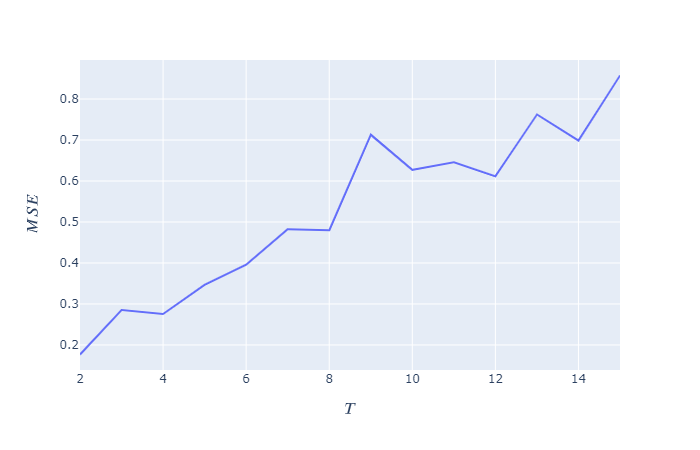
\includegraphics[scale=0.25]{day_1.png}
    }
    \quad
    \subfigure[日线\underline{~~}2预测结果]{
        \centering
        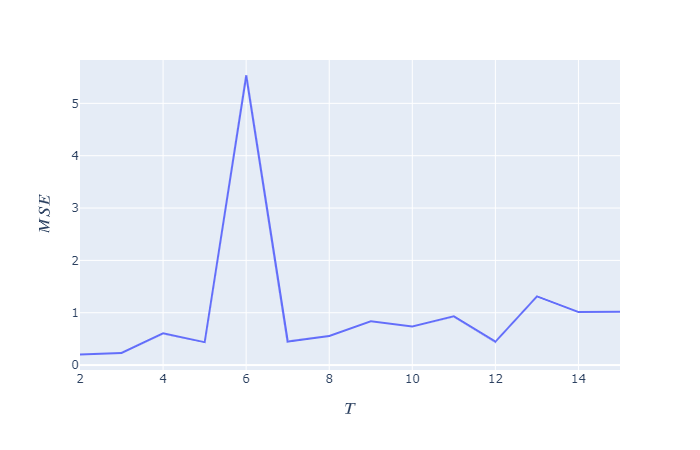
\includegraphics[scale=0.25]{day_2_old.png}
    }
    \quad
    \subfigure[周线\underline{~~}1预测结果]{
        \centering
        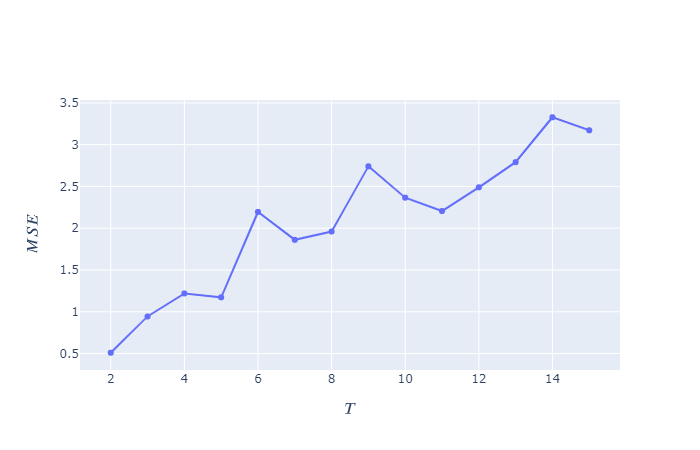
\includegraphics[scale=0.25]{week_1.png}
    }
    \quad
    \subfigure[周线\underline{~~}2预测结果]{
        \centering
        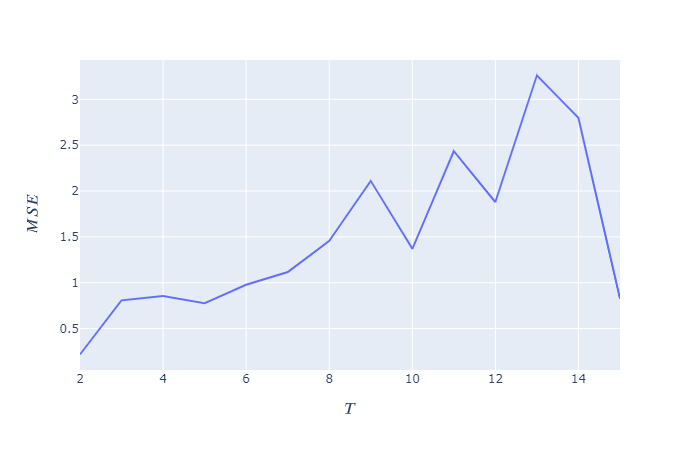
\includegraphics[scale=0.25]{week_2.png}
    }
\end{figure}

从图(4.1a)中我们可以看到$MSE$曲线比较曲折,但大体上是随着$T$的增加而增加的。
我们可依据预测结果作出如下推断:当今日成交量大于昨日成交量,且今日收盘价大于昨日收盘价的情况出现时,
适宜做短期投资,因为投资周期越小,所预测的未来$T$交易日最低价平均值就越准确。

\subsection{日线第2种情况}

\begin{figure}[htb]
    \centering
    \caption{日线\underline{~~}2预测结果}
    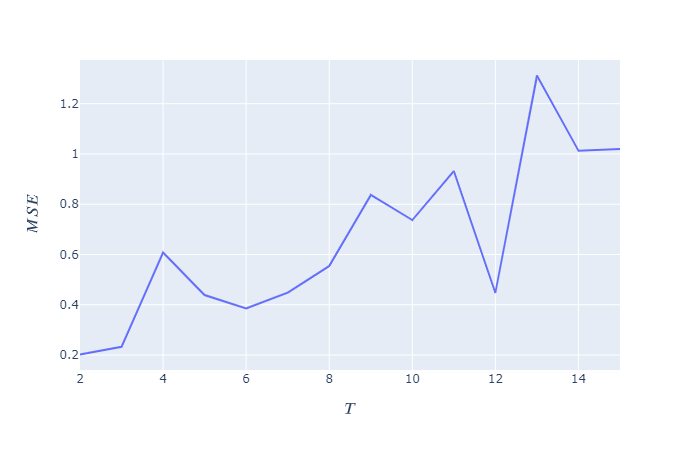
\includegraphics[scale=0.5]{day_2_new.png}
\end{figure}

图(4.1b)表明对于日线\underline{~~}2的预测结果波动较大,
模型在$T=7,8,9,10,12$时的预测表现均不错,
在$T=6$处出现了重大的预测误差,对投资行为十分不利,经过反复验证,
最终证明引起此处异常的股票代码为603318,在2016年6月28号前后,价格几近腰斩。
将此股票剔除后得到图(4.2)。

\subsection{周线第1种情况}

如图(4.1c),周线\underline{~~}1的预测结果波动不大,
其中$MSE$的最低值在$T=3$时出现而不是$T=2$,
另外在$T=9\sim13$区间$MSE$值比较平稳。

\subsection{周线第2种情况}

如图(4.1d),$MSE$曲线在$T$较高时有些曲折,但模型的总体表现非常好,
只有2处$T=11$和$T=13$劣于周线\underline{~~}1,
甚至在$T=2$时接近于日线\underline{~~}2的情况,
值得注意的是,在$T=15$处模型也取得了相当不错的预测结果。

\subsection{总结}

\begin{figure}[ht]
    \centering
    \caption{4种实验结果汇总}
    \subfigure[气泡图]{
        \centering
        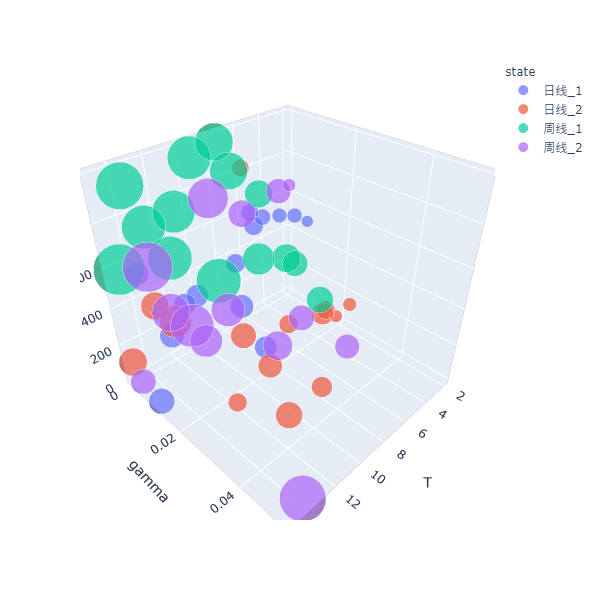
\includegraphics[scale=0.5]{3.png}
    }
    \quad
    \subfigure[预测误差汇总]{
        \centering
        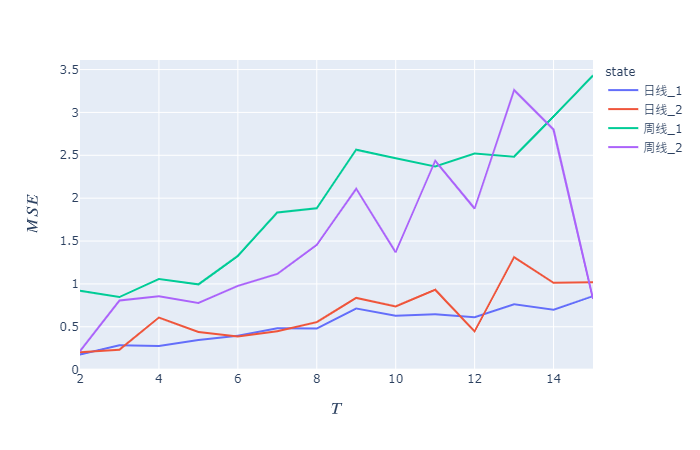
\includegraphics[scale=0.5]{sum.png}
    }
\end{figure}

在图(4.3a)中,每一个泡泡的大小代表$MSE$的大小,通过此图我们可以很清楚地认识到进行超参数寻优时黑盒函数的复杂性,
以及进行超参数寻优的必要性。

最后,我们将4种实验结果组合起来,如图(4.3b)。从图中我们可以观察到:
\begin{itemize}
    \item 周线\underline{~~}2的曲线最为曲折,且在$T=15$时取得比其余3种情况更优的结果。
    \item 除了周线\underline{~~}1,其余3种情况都是在$T=2$时取得$MSE$的最小值。
    \item 分别在$T=3,6,7,12$,日线\underline{~~}2的预测表现优于日线\underline{~~}1。
    \item 周线\underline{~~}1的预测误差仅在$T=11,13$时优于周线\underline{~~}1的结果。
\end{itemize}

通过对实验结果的总结,我们可以根据不同的情况给出投资建议:
\begin{enumerate}
    \item 当今日成交量大于昨日成交量,且今日收盘价大于昨日收盘价的情况出现时,即日线\underline{~~}1,投资周期越短预测越准确。
    \item 如果还出现了今日最低价小于昨日最低价的情况,即日线\underline{~~}2,选择投资周期$T=3,6,7,12\text{日}$,比日线\underline{~~}1更为准确。
    \item 当这周成交量大于上周成交量,且这周收盘价大于上周收盘价的情况出现时,即周线\underline{~~}1,选择投资周期$T=2,3,4,5\text{周}$和$T=9,10,11,12\text{周}$,预测结果比较平稳。
    \item 如果还出现了这周最低价小于上周最低价的情况,即周线\underline{~~}2,在大部分$T$上都取得了比周线\underline{~~}1更好的结果,尤其值得注意的是$T=2\text{周}$和$T=15\text{周}$,表现甚至优于日线。但是对于$8\text{周}\leq T\leq14\text{周}$,不建议以此投资周期进行投资。
\end{enumerate}